\paragraph{}
En \emph{Zycars} es posible añadir nuevos personajes por cualquier persona, siguiengo unos pasos muy sencillos,
sin necesidad de tocar una sola linea de código.

\paragraph{}
A continuación se detallan los distintos pasos que debemos llevar a cabo para añadir correctamente cualquier personaje que deseemos
al juego.

%%%%%%%%%%%%%%%%%%%%% IMAGENES NECESARIAS %%%%%%%%%%%%%%%%%%%%%%%
\section{Imagenes necesarias}

\paragraph{}
En primer lugar deberemos recopilar todas las imagenes necesarias para las distinas pantallas en las que sale el personaje, a 
continuación se explican las características que deben tener esas imagenes.

\paragraph{}
Anter de comenzar, dejar claro que todas las imagenes deben tener formato ''.png'', con cualquier otro formato se pueden tener 
problemas a la hora de ejecutar el juego.

\subsubsection{Vehículo del jugador}

\paragraph{}
Si duda la más importante de todas, ya que representará el vehículo que manejaremos en cualquiera de las carreras si elegimos al 
nuevo personaje añadido.

\paragraph{}
Por su puesto debe representar la imagen de un coche visto desde arriba, la imagen debe estar en horizontal con la parte delantera
del coche mirando hacia la derecha. La dimensiones que debe tener esta imagen son 47 píxeles de ancho y 24 píxeles de alto como 
máximo, cualquier imagen que tenga menor medida que las anterior dadas, no habrá ningún problema. Aunque hay que tener cuidado de no
añadir una imagen demasiado pequeña, para que se pueda ver correctamente. A continuación se muestra un ejemplo para que quede mas 
claro:

\begin{figure}[H]
  \label{ejemplo_coche}
  \begin{center}
    
\includegraphics[scale=1]{imagenes/ejemplo_coche.png}
  \end{center}
  \caption{Manual para añadir personajes: Ejemplo de coche con dimensiones de 42 x 18 píxeles.}
\end{figure}

\paragraph{}
Una vez que tenemos la imagen debemos añadirla a Zycars/multimedia/images/cars/.

\subsubsection{Imagen de corredor.}

\paragraph{}
Una vez añadido la imagen del vehículo del jugador, el siguiente paso es añadir la imagen que representará al jugador, hasta ahora 
la imagen de todos los corredores han tenido las siguientes características. En la imagen aparecen el corredor de cuerpo completo, 
junto con el vehículo que manejan. Aunque no es necesario que la imagen tenga esos componentes en concreto, pero se aconseja que sea
así para que no desentone con la imagen del resto de los corredores.

\paragraph{}
Otra cosa que debemos tener en cuenta es el tamaño de la imagen, en este caso la imagen debe tener unas medidas exactas y esta no
puede ser ni mayor ni menor, de se así se podría obtener malos resultados. El tamaño que debe tener la imagen es de 403 píxeles de
ancho por 246 píxeles de alto. A continuación un ejemplo:

\begin{figure}[H]
  \label{ejemplo_personaje}
  \begin{center}
    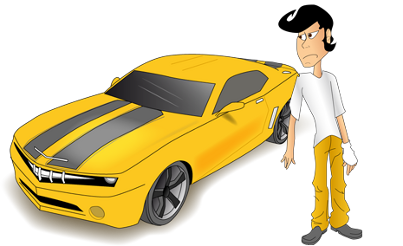
\includegraphics[scale=0.5]{imagenes/ejemplo_personaje.png}
  \end{center}
  \caption{Manual para añadir personajes: Ejemplo de imagen de corredo.}
\end{figure}

\paragraph{}
La imagen debemos añadirla a la carpeta Zycars/multimedia/image/character.

\subsubsection{Avatares del personaje}

\paragraph{}
Los avatares los usaremos para representar al jugador en el menú de selección, y también al jugador en carrera. Para ello son 
necesario dos avatares, ambas imagenes son idénticas y lo único que las diferencia son el tamaño que deben tener. La imagen debe
mostrar el rostro claro del corredor.

\paragraph{}
Para el avatar del menú de selección de personaje debe tener el tamaño de entre 150 y 90 píxeles de ancho y 149 píxeles de alto. 
Dichas medidas se deben cumplir de forma exhaustiva.

\paragraph{}
Para el avatar de carrera la imagen debe tener un tamaño de 67 y 42 píxeles de ancho y 69 píxeles de alto. Un ejemplo del avatar de 
un corredor seria el siguiente.

\begin{figure}[H]
  \label{ejemplo_avatar}
  \begin{center}
    
\includegraphics[scale=0.7]{imagenes/ejemplo_avatar.png}
  \end{center}
  \caption{Manual para añadir personajes: Ejemplo de avatar de corredor.}
\end{figure}

\paragraph{}
La imagen debemos añadirla a la carpeta Zycars/multimedia/image/character.

%%%%%%%%%%%%%%%%%%%%%% AÑADIR RECURSOS %%%%%%%%%%%%%%%%%%%%%%
\section{Añadir imagenes a los recursos del juego}

\paragraph{}
Una vez que hemos reunido todas las imagenes necesarias del nuevo corredor que deseamos añadir, el siguiente paso será indicar
dichas imagenes como recursos del juego para que se puedan usar sin problemas durante la ejecución de este.

\paragraph{}
Para ello debemos abrir el archivo llamado resources.xml que se encuentra en Zycars/xml, dicho archivo es muy extenso, ya que 
contiende todos los recursos que hace uso el juego, ya sean imagenes, sprites o sonidos.

\paragraph{}
En primer lugar añadiremos la imagen que representa al vehículo, buscamos <sprites>, y justo tras de ella añadimos la siguiente 
linea:

\begin{lstlisting}[style=XML]
<sprite code="new_car" name="cars/new_car.png" rows="1" columns="1" alpha="True"/>
\end{lstlisting}

\paragraph{}
Suponiendo que la imagen del vehículo del corredor se llama ''new\_car.png''. El atributo code, indica el código para acceder a 
dicho recurso, por lo que no se debe repetir.

\paragraph{}
El siguiente paso será añadir las imagenes referentes al personaje, como los avatares y el del personaje completo. Para ello en el 
fichero resources.xml buscamos la etiqueta <image> y añadimos las siguientes lineas tras esta:

\begin{lstlisting}[style=XML]
<image code="character_image" name="character/character_image.png" alpha="True"/>
<image code="big_avatar" name="character/big_avatar.png" alpha="True"/>
<image code="small_avatar" name="character/small_avatar.png" alpha="True"/>
\end{lstlisting}

\paragraph{}
Suponiendo que la imagen completa del personaje se llama ''character\_image.png'', el nombre del avatar grande sea 
''big\_avatar.png'' y el nombre del avatar pequeño sea ''small\_avatar.png''.

\paragraph{}
Una vez hecho esto ya hemos añadido todos los recursos necesarios que necesita el personaje. Debemos tener cuidado de nuevo con el
código de cada una de las imagenes y que no esteń repetidas en ningún otro recurso.

%%%%%%%%%%%%%%%%%%%%% CREACION FICHERO PERSONAJE %%%%%%%%%%%%%%%%%%%%55
\section{Creación del fichero del personaje}

\paragraph{}
El siguiente paso que deberemos llevar a cabo será crea el fichero del personaje donde indicaremos las principales características
de este como puede ser la velocidad, ángulo de giro, etc. La plantilla para dicho fichero será la siguiente:

\begin{lstlisting}[style=XML]
<car name_character="" sprite_code="" racer_image="" avatar="" max_speed="" 
min_speed="" aceleration="" desaceleration="" rotation_angle="">
<!--NORMAL, NOACTION, RUN, FORWARD, REVERSE, DAMAGED, ERASE, YAW-->
    <animations>
        <animation name="normal" frames="0" delay="1"/>
        <animation name="noaction" frames="0" delay="1"/>
        <animation name="foward" frames="0" delay="1"/>
        <animation name="run" frames="0" delay="1"/>
        <animation name="reverse" frames="0" delay="1"/>
        <animation name="damaged" frames="0" delay="1"/>
        <animation name="erase" frames="0" delay="1"/>
        <animation name="yaw" frames="0" delay="1"/>
        <animation name="fall" frames="0" delay="1"/>
        <animation name="turbo" frames="0" delay="1"/>
    </animations>
</car>
\end{lstlisting}

\paragraph{}
Sólo debemos preocuparnos de las dos primeras lineas en las que deberemos rellenar los siguientes atributos:

\begin{itemize}
    \item \textbf{name\_character}: En este atributo deberemos poner el nombre que tendrá nuestro personaje.
    \item \textbf{sprite\_code}: Aquí deberemos poner el código de la imagen que representará al vehículo del personaje.
    \item \textbf{racer\_image}: En este otro deberemos poner el código de la imagen que representa al jugador completo.
    \item \textbf{avatar}: Debemos poner el código del avatar que representará al jugador en carrera, es decir, 
    el del avatar pequeño.
    \item \textbf{max\_speed}: Velocidad máxima del personaje, su valor debe estar entre 5.7 y 6.5.
    \item \textbf{min\_speed}: Velocidad marcha atrás del personaje, valor entre 2.8 y 3.4.
    \item \textbf{aceleration}: Aceleración del vehículo, valor entr 0.1 y 1.
    \item \textbf{desaceleration}: Desaceleración del vehículo cuando no se acelera y ni se da marcha atrás. Valor 
    entre 0.05 y 0.1.
    \item \textbf{rotation\_angle}: Ángulo de rotación, valor recomendado entre 0.2 y 0.4.
\end{itemize}

\paragraph{}
Una vez completado el fichero del personaje, deberemos guardarlo con extension ''.xml'' y almacenarlo en el directorio
zycars/xml/cars.

\section{Añadir al personaje para que sea seleccionable.}

\paragraph{}
Tras todos los paso anteriores, el último paso para poder manejar y disfrutar del nuevo personaje que hemos añadido se
explica a continuación.

\paragraph{}
Nos vamos al fichero que se encuentra en zycars/xml/menu/charactermenu.xml y lo abrimos. Dentro de este buscamos la siguiente
linea:

\begin{lstlisting}[style=XML]
<characters normal_image='normal_box2' selected_image='selected_box2'>
\end{lstlisting}

\paragraph{}
Justo detrás de esta linea deberemos añadir otra linea que tenga la siguiente forma:

\begin{lstlisting}[style=XML]
<character image="" name='' image_car='' path_xml="cars/" 
speed='' aceleration='' rotation=''/>
\end{lstlisting}

\paragraph{}
Los distintos parametros que debemos completar se explican a continuación:

\begin{itemize}
    \item \textbf{image}: Código de la imagen del avatar grande que representa al personaje.
    \item \textbf{name}: Nombre del personaje, debe coincidir con el que añadimos en el fichero del personaje.
    \item \textbf{image\_car}: Código de la imagen que representa al jugador completa.
    \item \textbf{path\_xml}: Añadir el nombre del fichero con las características del jugador.
    \item \textbf{speed}: Velocidad del jugador para que se vea en el menú.
    \item \textbf{aceleration}: Aceleración del jugador para que se vea en el menú.
    \item \textbf{rotation}: Rotación del jugador para que se vea en el menú.
\end{itemize}

\paragraph{}
Una vez seguido todos los pasos anteriores, ya podremos disfrutar del nuevo jugador que hemos añadido.
